\chapter{Inleiding}
Voor het practicum OOPR1 zijn (ongeveer) 25 RockPi’s beschikbaar. Dit zijn Raspberry Pi achtige ‘Single Board Computers’ die met een Linux variant werken, in dit geval Debian 10. De RockPi’s zijn aangeschaft omdat Raspberry Pi’s niet leverbaar (of te duur) waren.
Tijdens het practicum gebruik je een RockPi van school. Je kunt deze alleen op school gebruiken, je mag hem niet meenemen naar huis. Dat is dan ook het belangrijkste nadeel.

Het gebruik van de RockPi heeft een aantal voordelen:
\begin{itemize}
\item Je hoeft zelf niets aan te schaffen
\item Je werkt onder gecontroleerde omstandigheden: de verstrekte RockPi bevat alles wat nodig is voor het practicum. Dat betekent dat jij- of de docent- niet eerst moet puzzelen om de omgeving aan de praat te krijgen.
\end{itemize}

\hypertarget{USBinleiding}{}
Bij het practicum heb je \textit{je eigen} USB stick nodig om je bestanden op te zetten (\textit{geen gedeelde!}). Een USB stick van 1GB is goed genoeg (128+ MB). Groter is zonde.
\begin{itemize}
\item Je werkt op je eigen \hyperlink{chp:USBstick}{USB stick} en niet op het bestandssysteem van de RockPi. 
\item Na afloop van het practicum lever je de RockPi in zonder daar bestanden op achter te laten. 
\item Ga er vanuit dat de RockPi’s na een practicum gewist worden!
\end{itemize}

\section{Voorbereiding - Software installeren}
Zorg dat je vóór het practicum de volgende software geïnstalleerd hebt:
\begin{itemize}
\item Installeer Github Desktop: \url{https://desktop.github.com/}
\item Vanuit Github Desktop, druk Ctrl+Shift+O voor 'Clone repository' en voeg de repository \textbf{JohnVi-hhs/oop} toe.
\item Installeer 'Visual Studio Code' (VSC) volgens de instructies in \newline \url{https://github.com/Grrtzm/OOPR1} \textit{(moet nog aangepast worden)}
\item Download en installeer de VNC viewer:  \newline \url{https://www.realVNC.com/en/connect/download/combined/}
\item (Optioneel maar wel handig) Download en installeer de SSH client KiTTY  \newline \url{https://www.fosshub.com/KiTTY.html} \newline
KiTTY is een opvolger van PuTTY. Het grote voordeel is dat KiTTY automatisch opnieuw verbinding maakt als de verbinding even verbroken is geweest.
\end{itemize}

\section{Eerste gebruik van de RockPi}
We gaan er van uit dat je de RockPi in lokaal D2.001 of D2.003 van HHS Delft gebruikt. \newline
De RockPi is al ingesteld voor Wi-Fi netwerk in D2.001: \textbf{Lab001}. \newline
Log ook met je laptop in op dit netwerk. Het password is \textbf{Lab001WiFi}. \newline
In Figuur \ref{fig:netw} wordt weergegeven hoe de RockPi op het lab netwerk is aangesloten.
\begin{figure}[h!]
	\centering
	\begin{center} 	
		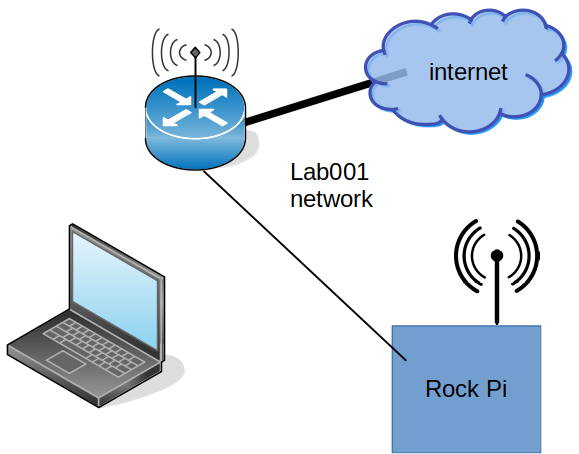
\includegraphics[width=0.4\textwidth]{figuren/laBnetwork}
		\caption{De RockPi in het lab netwerk}
		\label{fig:netw}   
	\end{center}
\end{figure}
\break
Sluit de USB-C voedingskabel aan zodat de RockPi gaat opstarten (op de RockPi gaat een groene led branden). Verder hoef je nog niets aan te sluiten!
\begin{figure}[h!]
	\centering
	\begin{center} 	
		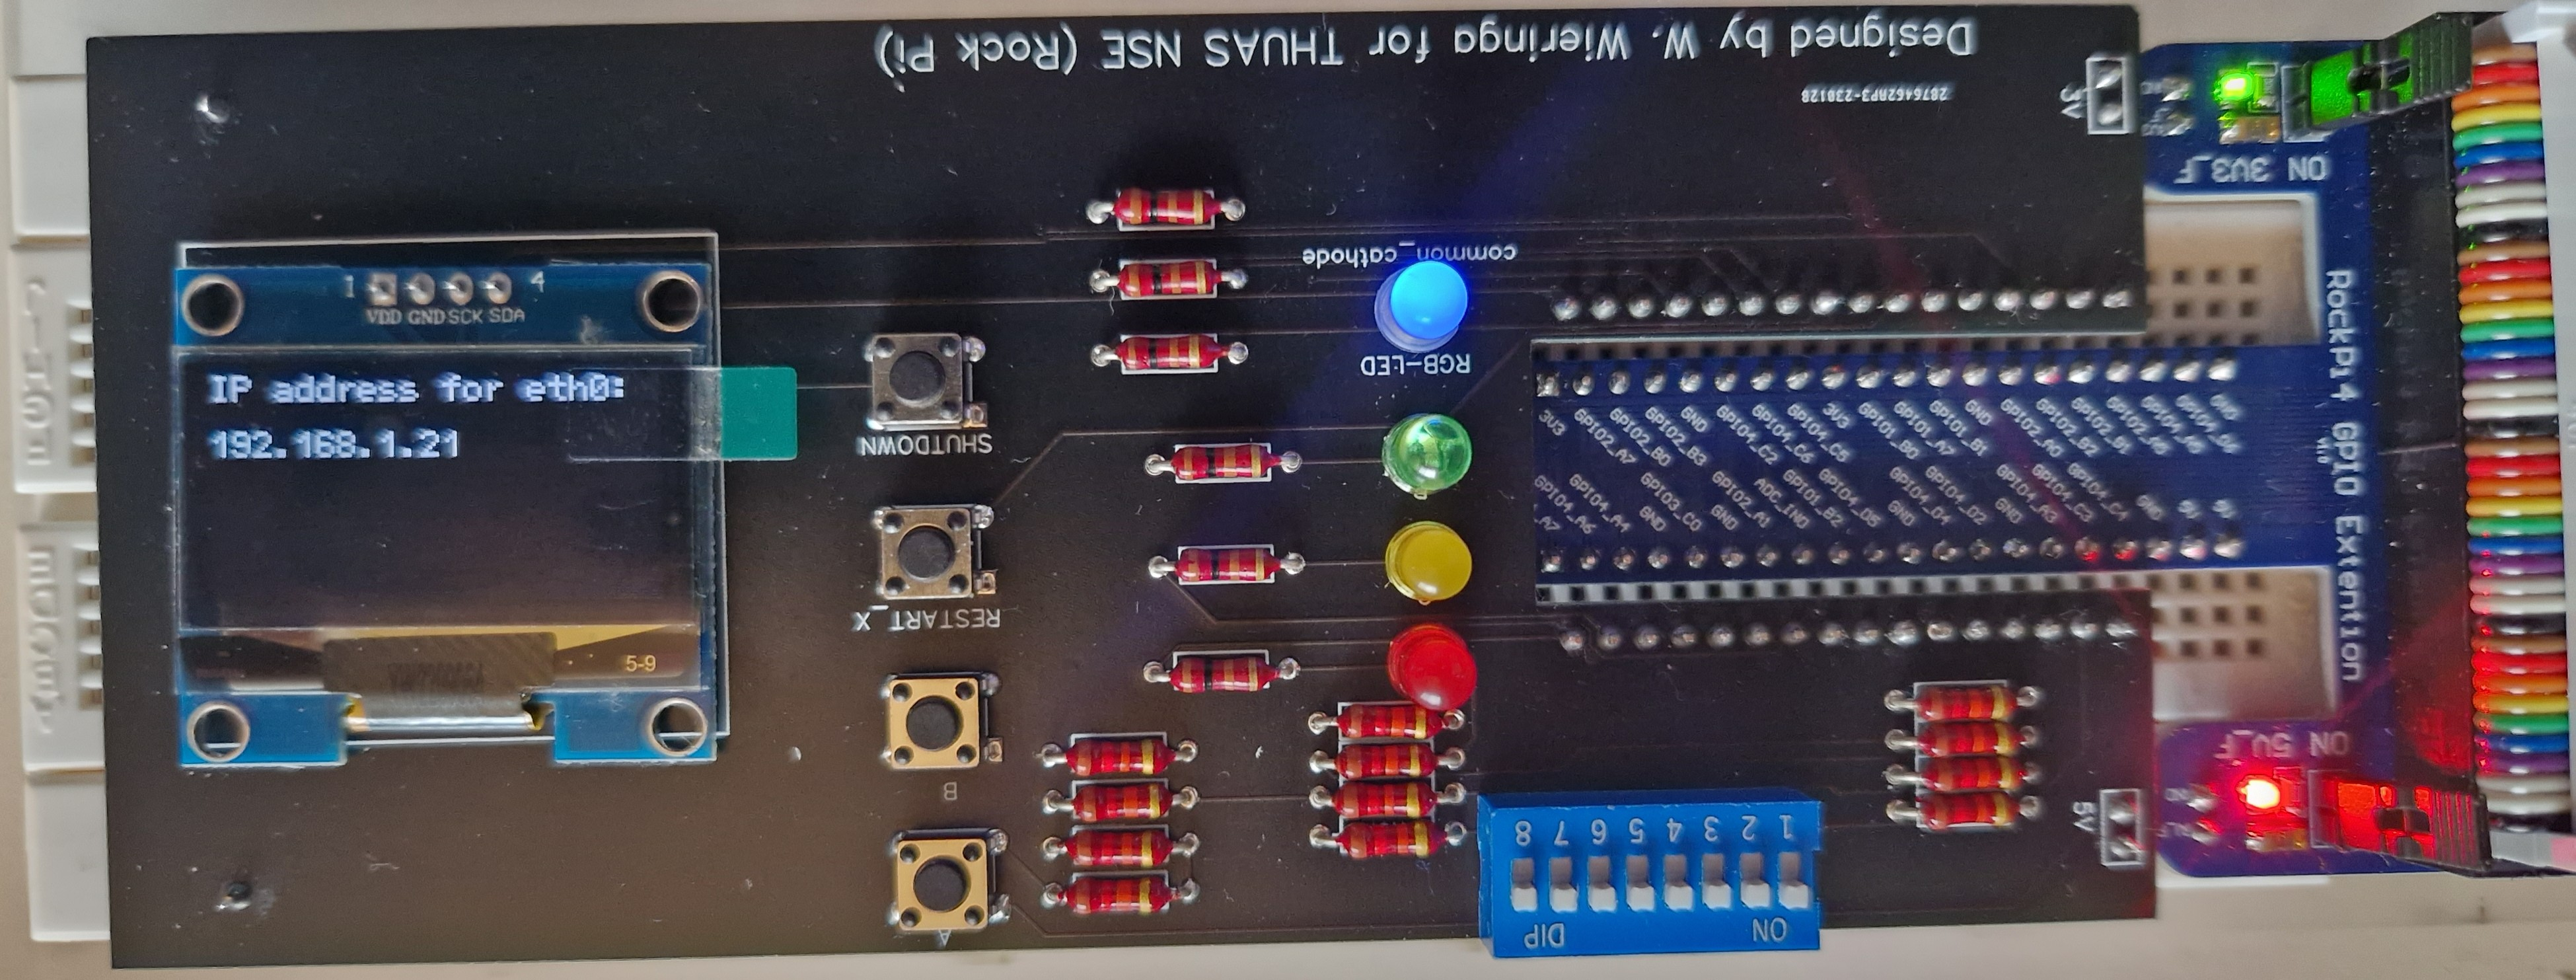
\includegraphics[width=1\textwidth]{figuren/rockIPnr}
		\caption{Het uitbreidingsbord van de RockPi}
		\label{fig:rockIPnr}   
	\end{center}
\end{figure}

\textbf{\textit{Controleer de zelftest:}} Om zeker te weten dat het bovenstaande bordje OK is gaat de RockPi alle leds even aan en uitzetten. \newline
Als je de RockPi in het lab (D2.001) aanzet, verschijnt op het oled display bij “IP address for wlan0:” een IP adres van het Lab001 Wi-Fi netwerk (zie Figuur \ref{fig:rockIPnr}). \newline
Nu kun je via SSH en/of VNC een verbinding maken met dit IP adres en inloggen op de RockPi.
De username is \textbf{rock}, het password is ook \textbf{rock}. Mocht er een sudo password gevraagd worden, dan is dit ook \textbf{rock}.
Overigens kun je ook een ethernet kabel aansluiten zoals in Figuur \ref{fig:rockIPnr} te zien is bij “IP address for eth0:”.\break\newline
Zorg wel dat je PC op hetzelfde netwerk is aangesloten. Als VNC het niet wil doen, maar ssh wel, dan zitten je PC en de RockPi mogelijk op verschillende Wi-Fi access-points. Als VNC niet werkt, maar je RockPi en laptop zitten wel op hetzelfde netwerk, dan kun je het knopje '\textbf{Restart\_X}' indrukken, dit herstart de grafische schil op de RockPi.

Zodra je bent ingelogd met VNC, kun je je USB stick aansluiten en configureren. Het maakt niet uit welke USB poort je gebruikt. 

Als je klaar bent met je practicum, moet je de RockPi netjes afsluiten. Door op het knopje ‘\textbf{Shutdown}’ te drukken, wordt het operating system netjes afgesloten zodat het bestandssysteem niet corrupt raakt (wat kan gebeuren als je de RockPi gewoon uitzet).

'Knop\_A' kun je gebruiken om tijdens het opstarten voor volledig GPIO gebruik te kiezen; druk de knop in vóórdat je de RockPi aanzet, en houd hem ingedrukt tot de LED zelftest klaar is. Dit is zo gedaan omdat wisselen tussen PWM gebruik (voor de rode en blauwe leds van de driekleuren led) en GPIO (alleen aan en uit, geen ‘analoge’ waarden) niet lukt zonder opnieuw op te starten.

Aan 'Knop\_A', 'Knop\_B' en de DIP switches (blauwe blokje) zijn verder geen functies toegewezen. Daar kun je zelf code voor schrijven.

\section{Inloggen met VNC}
Voer het IP adres zoals getoond op het oled display in op VNC (Figuur \ref{fig:rockIPnr}).\newline
Log in op de RockPi en klik op het ‘Terminal’ icoon (rood omcirkeld in Figuur \ref{fig:termico}):
\begin{figure}[h!]
	\centering
	\begin{center} 	
		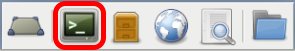
\includegraphics[width=0.4\textwidth]{figuren/Terminal-icoon}
		\caption{Terminal icoon}
		\label{fig:termico}   
	\end{center}
\end{figure}

Nu verschijnt het Terminal venster. Van hieruit kun je allerlei commando's invoeren:
\begin{figure}[h!]
	\centering
	\begin{center} 
		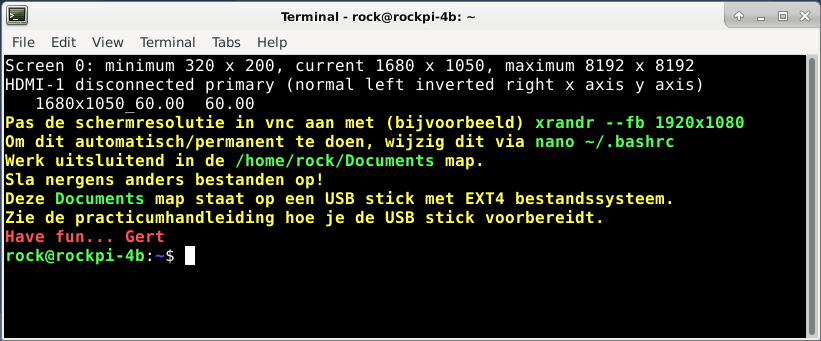
\includegraphics[width=0.9\textwidth]{figuren/terminal-inlogscherm}	
		\caption{Het Terminal scherm}
		\label{fig:terminal-inlogscherm}   
	\end{center}
\end{figure}

\hypertarget{chp:USBstick}{}
\section{USB Stick voorbereiden}
\textbf{\textit{LET OP!! }}
\begin{itemize}
	\item Met onderstaande procedure verwijder je alle bestanden van je USB stick!
	\item Je hebt genoeg aan een \hyperlink{USBinleiding}{kleine USB stick} (ergens tussen 128MB en 4 GB).
	\item Je kunt hierna alléén met Linux op je USB stick kijken, niet meer met Windows!
\end{itemize}

Formatteer nu je USB stick met EXT4 filesystem. Dit is nodig omdat Linux d.m.v. attributen in het bestandssysteem aangeeft of een bestand uitvoerbaar (‘executable’) is. Dat is op  een Windows compatible USB stick (met FAT of NTFS bestandsysteem) niet mogelijk.
Kijk of je USB stick gezien wordt. Geef het commando \textbf{\texttt{lsblk}} en kijk of daar een device bij zit met sda in de naam (zie hieronder in de listing van \texttt{lsblk}). In dit geval is deze er. De partitie waar we gebruik van maken is /dev/sda1.

\begin{lstlisting}[language=bash]
rock@rockpi-4b:~$ lsblk
NAME         MAJ:MIN RM   SIZE RO TYPE MOUNTPOINT
sda            8:0    1   1.9G  0 disk
`-sda1         8:1    1   1.9G  0 part /media/rock/9C02-C2F1
mmcblk1      179:0    0 115.2G  0 disk
|-mmcblk1p1  179:1    0   3.9M  0 part
|-mmcblk1p2  179:2    0     4M  0 part
|-mmcblk1p3  179:3    0     4M  0 part
|-mmcblk1p4  179:4    0   512M  0 part
`-mmcblk1p5  179:5    0   7.8G  0 part /
mmcblk1boot0 179:32   0     4M  1 disk
mmcblk1boot1 179:64   0     4M  1 disk
mmcblk1rpmb  179:96   0     4M  0 disk
}
\end{lstlisting}
	
\underline{\textbf{Controle:}}\newline 
Als je het commando \href{https://www.techrepublic.com/article/linux-101-what-is-the-mount-command-and-how-do-you-use-it/}{\textbf{\texttt{mount}}} geeft, dan verwacht je in de uitvoer het device (de disk) /dev/sda1 te zien: % \textbf{\texttt{mount}}
\begin{lstlisting}
/dev/sda1 on /media/rock/9C02-C2F1 type vfat (rw,nosuid,nodev,relatime,uid=1000,gid=1000,fmask=0022,dmask=0022,codepage=936,iocharset=utf8,shortname=mixed,showexec,utf8,flush,errors=remount-ro,uhelper=udisks2)
\end{lstlisting}

Hierboven zie je dat disk ge-'mount' is. Om te formatteren moet je eerst 'umount' doen:\newline
\textbf{\texttt{umount /dev/sda1 }}\newline
Nu USB disk formatteren met ext4 filesystem (sudo password is \textit{rock}):\newline
\textbf{\texttt{sudo mkfs -t ext4 /dev/sda}}\newline
Vervolgens disklabel 'Documents' instellen:\newline
\textbf{\texttt{sudo e2label /dev/sda Documents}}\newline
Als laatste gebruiker \textit{rock} eigenaar maken van de USB stick:\newline
\textbf{\texttt{sudo chown rock /home/rock/Documents}}\newline

Hieronder zie je de output van bovenstaande commando's:
	
\begin{lstlisting}[language=C]   % Gert: Is het niet, maar hiermee doet hij geen speciale opmaak
rock@rockpi-4b:~\$ umount /dev/sda
umount: /dev/sda#: No such file or directory
rock@rockpi-4b:~\$ sudo mkfs -t ext4 /dev/sda
mke2fs 1.44.5 (15-Dec-2018)
/dev/sda contains a vfat file system
Proceed anyway? (y,N) y
Creating filesystem with 491520 4k blocks and 123120 inodes
Filesystem UUID: 1b2275ec-6dbd-4f3b-8d41-feaf4da0c7b7
Superblock backups stored on blocks:
32768, 98304, 163840, 229376, 294912

Allocating group tables: done
Writing inode tables: done
Creating journal (8192 blocks): done
Writing superblocks and filesystem accounting information: done
\end{lstlisting}

Als het formatteren en labelen klaar is, kun je testen of de USB stick correct gezien wordt:\newline
Verwijder de USB stick, wacht even en steek hem weer terug in een USB poort.\newline
Klik in VNC op het ‘File Manager’ icoon (rood omcirkeld in Figuur \ref{fig:fileman}):

\begin{figure}[h!]
	\centering
	\begin{center} 	
		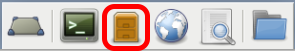
\includegraphics[width=0.4\textwidth]{figuren/File-Manager}
		\caption{Terminal icoon}
		\label{fig:fileman}   
	\end{center}
\end{figure}
Ga in de ‘File Manager’ naar het ‘Documents’ device.\newline
Als dit werkt, dan zie je onderin de statusbalk van de ‘File Manager’ hoeveel vrije ruimte je USB stick heeft (rood omcirkeld in Figuur \ref{fig:fileman})

\begin{figure}[h!]
	\centering
	\begin{center} 	
		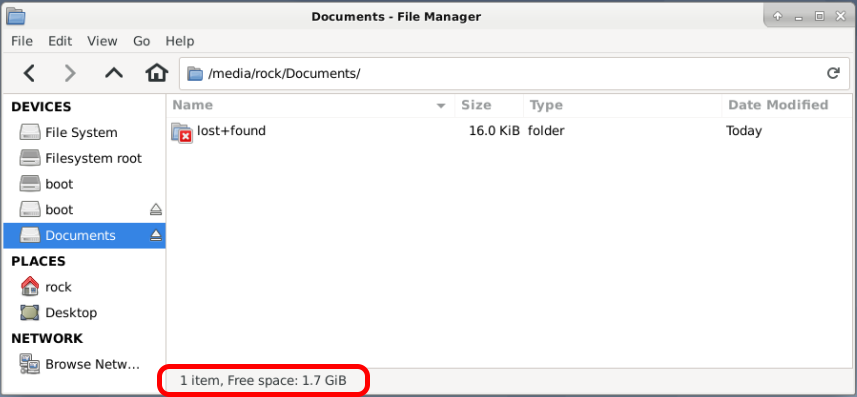
\includegraphics[width=1\textwidth]{figuren/FileManagerUsbStick}
		\caption{File Manager}
		\label{fig:FileManagerUsbStick}   
	\end{center}
\end{figure}

Met de 'File Manager' kun je in het bestandssysteem van Linux kijken.\newline
Bij het practicum werk je alleen maar in de home directory en subdirectories van gebruiker \textbf{rock} (\texttt{/home/rock}).\newline
Als je meer wilt weten over het Linux bestandssysteem, \href{https://www.techrepublic.com/article/linux-101-demystifying-the-linux-directory-structure/}{klik dan hier}.
